\chapter{Strategies Evaluation}
\label{chap:strategies}

\section{Modelisation}
\subsection{Metrics}
A way to rationaly compare strategies is needed in order to discuss their
relative strengths and weaknesses. Three main characteristics will be used for
that:
\begin{itemize}
        \item latency;
        \item number of nodes;
        \item overhead.
\end{itemize}

\subsubsection{Latency}
The latency is the number of messages needed to finalize a block. Ideally, you
want to have a latency as low as possible to reach finality as soon as possible.
The latency is a way to measure liveness in a blockchain system. If it is low,
then the system is considered more "live", as fewer messages are needed in order
to confirm a transaction, and therefore less time.

\subsubsection{Number of nodes}
The number of nodes is quite straightforward; it is the number of nodes that are
in the validator set. This number should be as high as possible to guarantee
decentralization and therefore safety.

\subsubsection{Overhead}
The overhead is the number of messages that are sent over the network between
one step of the consensus and the next. It should be as low as possible to keep
the costs in bandwidth low.

\subsubsection{Example}

\begin{figure}[H]
	\centering
	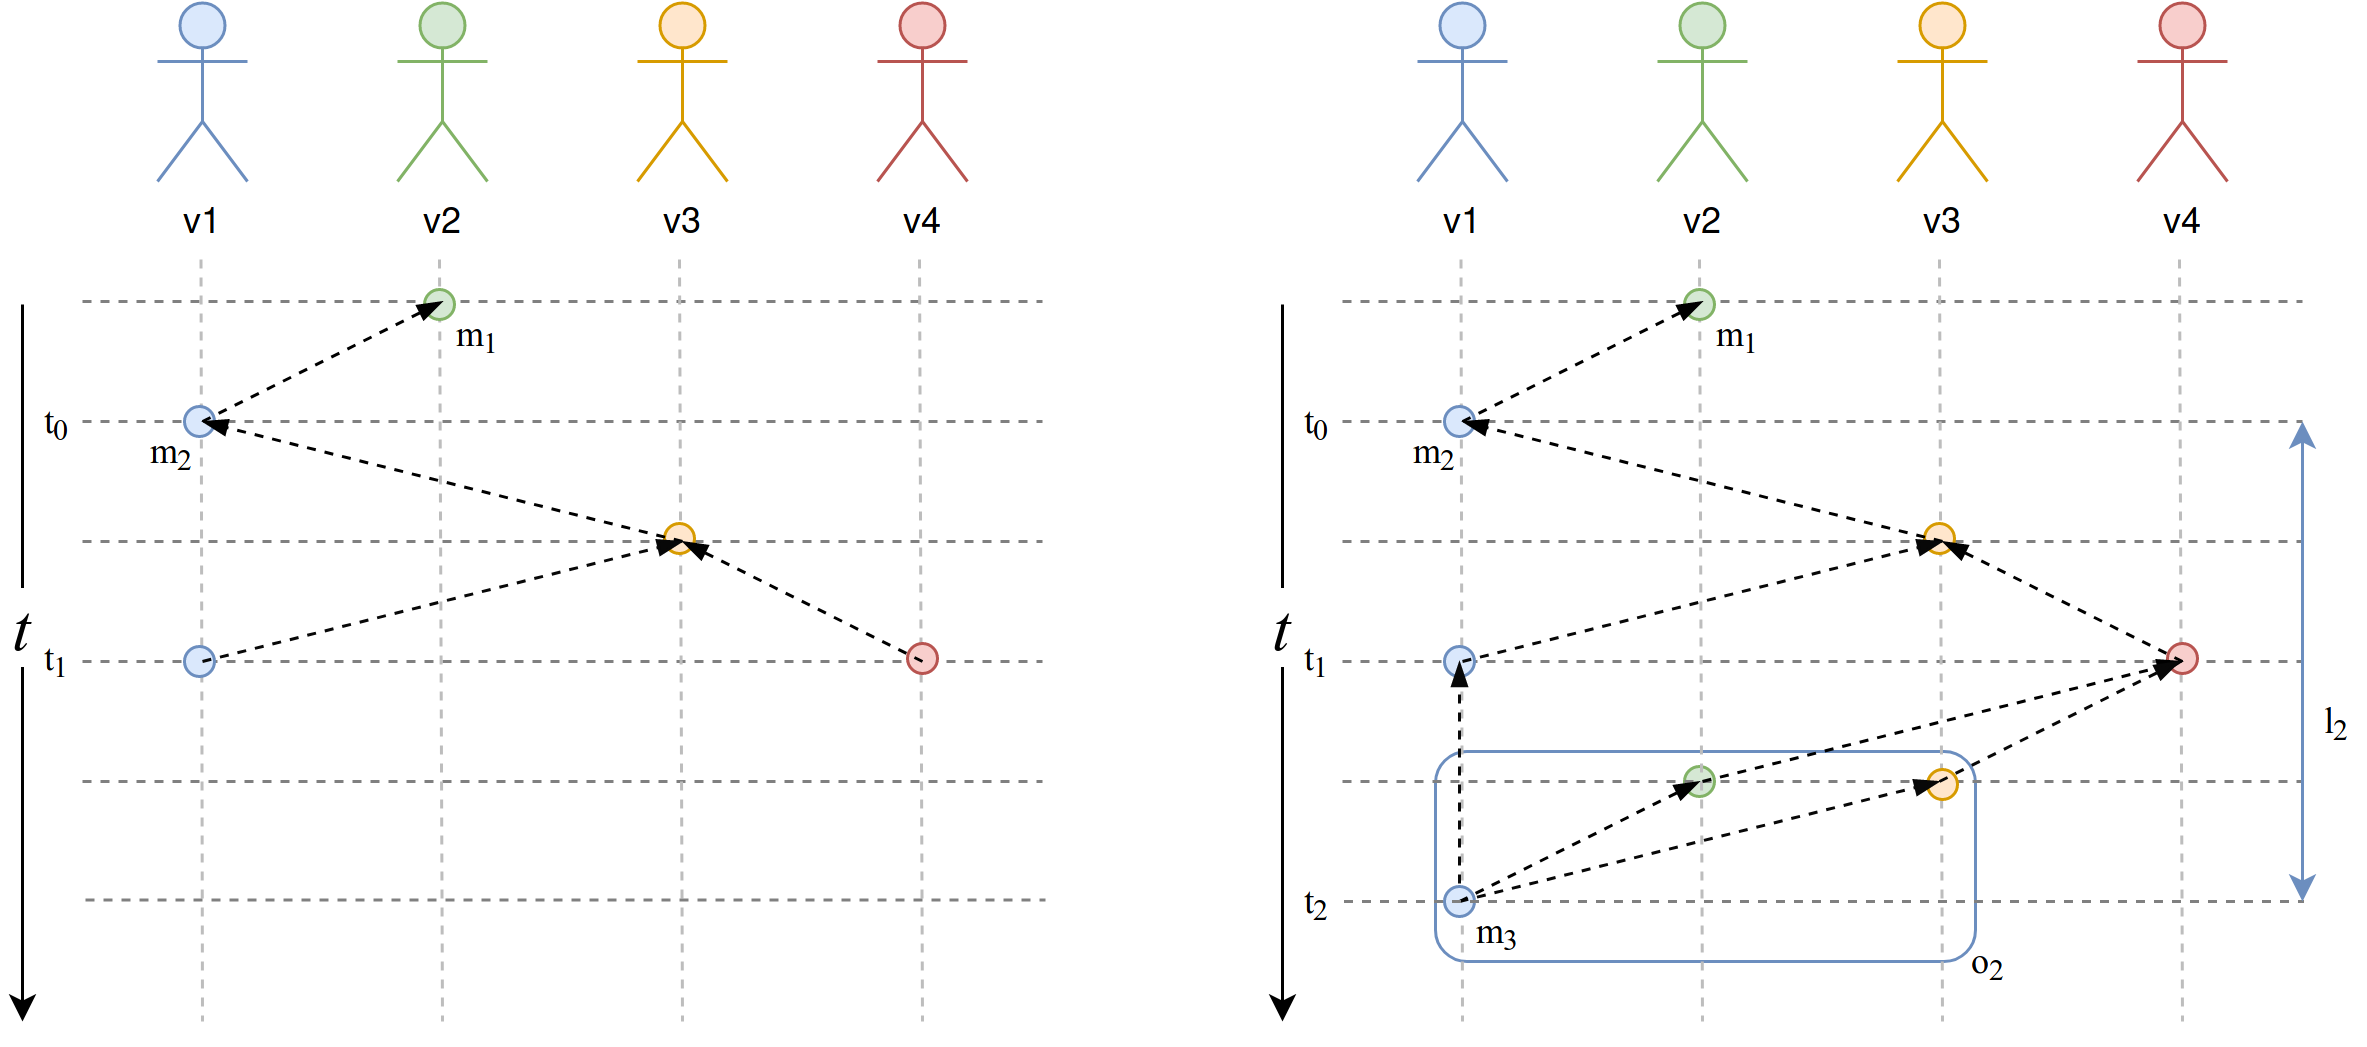
\includegraphics[width=\columnwidth]{metrics-example}
  \captionsetup{justification=centering}
    \caption{Metrics computation example}
	\label{fig:metricsSchema}
\end{figure}

Figure~\ref{fig:metricsSchema} describes how the computation of the metrics
takes place. The left half of the figure shows an initial view of the system. At
time \(t_1\), message \(m_1\) is finalized. The right half of the figure shows a
view of the system at \(t_2\), time at which \(m_2\) is finalized. The latency
of \(m_2\) is \(l_2\), the difference of heights between \(m_3\) and \(m_2\). In
this example, \(l_2 = 4\). \(o_2\), the overhead for \(m_2\), is the number of
messages that have been sent between \(t_1\) and \(t_2\), \(t_1\) being the time
at which the previous message has been finalized and \(t_2\) the time at which
the current message is finalized. In the example, \(o_2 = 3\).

\subsection{Tradeoff triangle/Trilemma}
In a standard consensus protocol, the three metrics form a trade-off triangle in
kind of a "pick two" fashion. \todo{not a pick two} \gls{cbc}-Casper has no
assumptions on timings, sources, contents, destinations of the messages that are
exchanged, and can therefore explore the whole trade-off space. This project
aims to find strategies that span the entierty of the triangle and 
\todo{finish sentence what}

\subsection{Basic model}
\label{ssec:model}
The first model that has been chosen for the evaluation is the following:

\[1 = s_n \cdot \frac{1}{n} + s_l\cdot l + s_o\cdot o\]

This model binds 3 scores \(s_x\) to their respective variables \(x\).
Variables are as follows:
\begin{itemize}
    \item \(n\) the number of nodees;
    \item \(l\) the latency;
    \item \(o\) the overhead.
\end{itemize}
The higher the score \(s_x\) is, the more its related variable is dominant
in the strategy and therefore the closer to a corner of the triangle the strategy is.
\(\frac{1}{n}\) is used because a large number of nodes is wanted.
This model is a basic one, where everything is linear. It is probably not accurate but
will serve as a base for a closer to reality one once data have been plotted using
this model.
\todo{why 1/n, why everything linear?}

\subsection{Model Evaluation}
After running the strategies in the simulation environment, metrics for \(n\),
\(l\) and \(o\) will be recorded. Then, for multiple runs, a linear regression
will be performed in order to find the scores \(s_x\).

\section{Strategies}
\label{sec:strategies}

The following strategies were proposed in order to visit the entierty of the
trade-off triangle:
\begin{itemize}
        \item round-robin;
        \item randomness;
        \item double round-robin;
        \item triple round-robin;
        \item overhead.
\end{itemize}
These strategies should allow one to visit the whole triangle and to discuss
their respective strength and weaknesses. The following sections describe the
strategies as well as their expected locations in the triangle.

\subsection{Round-robin}
The first strategy that comes to mind is a simple round-robin. Nodes send
messages one after the other, in a fixed order.
\todo{talk about real life implications? aka synchronize all nodes?,\ldots and
that for every strategy}

\subsection{Randomness}
The next strategy is the simplest to think of: complete randomness. Using fixed
probability density functions, nodes chose when to create messages and to which
other validator to send them.

\subsection{Double Round-robin}
In this setting, two nodes send messages at the same time, in a fixed order. If
the two nodes that send messages at the same step are at opposite places in the
set of validators \todo{explain better}, the latency to finality is supposedly
half as much as the simple round-robin strategy. The overhead is however
doubled.\todo{add that we could have a triple rr, quadrr, \ldots}

\subsection{Triple Round-robin}
This strategy is similar to the Double round-robin, except that three nodes send
a message a each step. It was decided to add this strategy at a later stage of
the project in order to have intermediate comparison points between the Double
round-robin and the Maximal overhead strategy. As for the Double round-robin
strategy, the latency should be divided by three compared to the simple
round-robin and the overhead should be three times higher.

\subsection{Maximal Overhead}
This strategy is the most expensive in terms of bandwidth; at each step, each
validator sends a message to the others. This example strategy should give a
baseline value for the maximum overhead that is reachable in the tradeoff
triangle.

\subsection{Bottom-up strategies}
All the previous strategies (except the Arbitrary one) can be viewed as
"top-down" strategies, as there has to be a way for nodes to be synchronized.
Strategies that are easier to implement from a real-life point of view would be
strategies that only depend on the data available on a node. For exemple, a node
could keep track of the whole state of the finalization of messages, and only
publish a message itself when it facilitates the finalization. That kind of
strategy has not been implemented but the testing and scoring framework allows
one to easily add them.

Such strategies should implement incentives for the nodes not to spam the
network and include mechanisms to slash nodes not following some rules the
strategies dictate.

\section{Experimentations}
Over the duration of this thesis, the \texttt{core-cbc} library has included a
test framework called \texttt{proptest}. The testing framework that has been
implemented includes ways to simulate the behavior of the Casper protocol over
multiple nodes and thousands \todo{numbers} of blocks. At the time of the
writing, the simulations do not include networking latencies.

\subsection{\texttt{proptest}}
The \texttt{proptest} implementation is able to run blockchain simulations off
the following parameters:
\begin{itemize}
    \item Number of validators;
    \item Terminating condition;
    \item Sender strategy;
    \item Receiver strategy.
\end{itemize}

\subsubsection{Number of validators}
This parameter is quite straightforward, it is the number of nodes that can
validate blocks.

\subsubsection{Terminating condition}
The terminating condition is a predicate that tells whether or not the simulation has
reached an end. In our case, the end of the simulation is reached when at least
one node finds a safety oracle for a blockchain that has an height of 4.
\todo{why 4}

\subsubsection{Sender strategy}
The sender strategy selects one or more nodes that will create new messages and
forward them to the rest of the network. All the basic strategies that have been
presented in Section~\ref{sec:strategies} are implemented as Sender strategies.
New strategies (including bottom-up ones) can be easily implemented as well.

\subsubsection{Receiver strategy}
Receiver strategies select a set of validators that receive messages created by
Sender strategies. Two strategies have been implemented for now: 
\begin{itemize}
        \item All receivers;
        \item Some receivers.
\end{itemize}

The \textit{all receivers} strategy broadcasts messages to each other validator.
The \textit{some receivers} strategy sends a message to \(1\) or more validator,
using an uniform probability density function.  As of now, none of the
implemented strategies are a good modelisation of a typical Ethereum network and
this will be fixed at a later iteration.  Nonetheless, these strategies offer
two extreme points on the spectrum of the network topology: a fully connected
one without latency (\textit{all receivers}), and a random one (\textit{some
receivers}) and will be both taken into account to compare the sender
strategies.

\subsection{Metrics measurements}
Metrics are not computed as-is in the \texttt{proptest} implementation. Simpler
datas are logged into \texttt{csv} files, and are processed by a \texttt{Python}
script. \todo{what data} This two steps processing permitted the generation of
data before having a precise definition of the metrics. It also permits to vary
the way metrics are recorded. For example, from the same log file, you could
extract metrics only when the last step of the consensus is reached, or have an
average of the metrics at each step of the consensus.

\subsection{Tests}
Table~\ref{fig:recapTests} summarizes which tests have been run.
All of them have the same terminating condition, which is reached when at least a
node finds a safety oracle at height 4. The number of nodes is chosen at random
in the interval \([1, 20[\). It has been decided to perform tests on this
interval because it is large enough to give an insight on the behavior of the
relations between the metrics, and small enough to reach the terminating condition in
a reasonable time (1 run with a number of nodes chosen at random takes on average 1 hour
with the Maximal overhead strategy).

\todo{renove table}

\begin{table}[H]
    \centering{
        \begin{tabular}{|c|c|c|}
            \hline
            & All receivers & Some receivers \\
            \hline
            Round-robin & \checkmark & \checkmark\\
            \hline
            Double round-robin & \checkmark & \checkmark\\
            \hline
            Maximal overhead & (\checkmark) & (\checkmark) \\
            \hline
            Arbitrary & \checkmark & \checkmark\\
            \hline
        \end{tabular}
        \captionsetup{justification=centering}
        \caption{Summary of tests that have been run. A tick in parenthesis
        implies that tests were run but that there are not many data points or
        big disparities in the distribution of the number of nodes}
        \label{fig:recapTests}
    }
\end{table}

\todo{schema with what to measure}
\todo{how the measurements take place in the code}

\section{Visualization I: All receivers}
This chapter presents a visualization of the datas obtained through the multiple
test runs with the All receivers strategy.  Each subsection shows the results
using 3 histograms, representing the raw data, followed by 3 scatter plots
picturing each metric against each other. These graphs also show a simple linear
regression as an attempt to find a relation between each metric. At the end of
the discussion of each strategy a linear regression is performed in order to
find the scores of each variable according to the model presented in
Subsection~\ref{ssec:model}.


\todo{3D plotting?}
\todo{undersampling issue?}

\subsection{Round-robin}

The distributions of the number of nodes and the latency
(Figure~\ref{fig:distRR} left and center) have the same
shapes except for the gaps every 3 steps. The resemblance in shape is explained
by the fact that the latency is strictly correlated to the number of nodes, as
expected.
The gaps will be explained in the next section, using the graphs that show
relations between variables. \todo{explain gaps}

\todo{fix center/left/right in captions and text}
\triplefigure
    {hist_nb_nodes_rr_20_nodes_4_depth_all_receivers_gen_averages}
    {hist_latency_rr_20_nodes_4_depth_all_receivers_gen_averages}
    {hist_overhead_rr_20_nodes_4_depth_all_receivers_gen_averages}
    {Distributions of the dataset. Number of nodes (left), latency (center)
    and overhead (right) \todo{change xticks label frequency}}
    {fig:distRR}

The histogram for the overhead is easy to analyse as well; the overhead is
expected to be 1 because once consensus is obtained for the genesis block, only
one message from the next validator is needed to finalize the next block.

\triplefigure
    {relation_nb_nodes_latency_rr_20_nodes_4_depth_all_receivers_gen_averages}
    {relation_nb_nodes_overhead_rr_20_nodes_4_depth_all_receivers_gen_averages}
    {relation_overhead_latency_rr_20_nodes_4_depth_all_receivers_gen_averages}
    {Relations between all the variables. Latency/Number of nodes (left),
    Overhead/Number of nodes (center) and Latency/Overhead (right)}
    {fig:relRR}

The right and center graphs on Figure~\ref{fig:relRR} do not give more insight on the
data, as the Overhead is always \(1\). On the other hand, the graph on the left
shows a clear linear relationship between the latency and the number of nodes.
The fitted line has the following equation:
\[l = 1.403402\cdot n\]
The latency is expected to be around \(1.5\cdot n\) because the finality is
reached when at least 50\% of the network has acknowledged that the whole
network has the finalized message in its justification. As pictured in the
top-left graph of Figure~\ref{fig:relRR}, the fitted line has a slightly small
slope compared to the data points due to the fact that the line is fitted to be
linear and the data points are close the origin. \todo{insert line with 1.5*n ?}

\subsection{Double round-robin}
\triplefigure
    {hist_nb_nodes_double_rr_20_nodes_4_depth_all_receivers_gen_averages}
    {hist_latency_double_rr_20_nodes_4_depth_all_receivers_gen_averages}
    {hist_overhead_double_rr_20_nodes_4_depth_all_receivers_gen_averages}
    {Distribution of the dataset. Number of nodes (left), latency (center)
    and overhead (right)}
    {fig:distDRR}
As for the simple round-robin case, the latency and number of nodes
distributions show a similar shape. The latency is less spread than for the
singl round-robin, which explains some dissimilarities between the
distributions. The distribution of the overhead presents a peak at 2, which is
expected but also shows that there are some messages that have double this
overhead, at 4. This will be explained using the following graphs. \todo{explain
outliers}

\triplefigure
    {relation_nb_nodes_latency_double_rr_20_nodes_4_depth_all_receivers_gen_averages}
    {relation_nb_nodes_overhead_double_rr_20_nodes_4_depth_all_receivers_gen_averages}
    {relation_overhead_latency_double_rr_20_nodes_4_depth_all_receivers_gen_averages}
    {Relations between all the variables. Latency/Number of nodes (left),
    Overhead/Number of nodes (center) and Latency/Overhead (right)}
    {fig:relDRR}

As for the simple round-robin strategy, the plots including the Overhead are not
of much use here, except they show that its value is 2, as it is expected. 
On the other hand, the plot on the top-left of Figure~\ref{fig:relDRR} shows a
linear relation between the number of nodes and the latency: 
\[l = 0.721750 \cdot n\]
This value is about half of the slope obtained for the same relation with the
round-robin strategy. The double round-robin strategy was supposed to show half
the latency with respect to the simple round-robin and this value is therefore
correct. The value of 2 for the overhead is also twice the overhead for the
single round-robin and confirms the hypothesis.
    

\subsection{Triple round-robin}
The triple round-robin strategy shows  the same kind of information as the
double round-robin one. The overhead is 3 for almost all cases (this will be
discussed later), and the number of nodes and latency are lineraly correlated.
\triplefigure
    {hist_nb_nodes_triple_rr_20_nodes_4_depth_all_receivers_gen_averages}
    {hist_latency_triple_rr_20_nodes_4_depth_all_receivers_gen_averages}
    {hist_overhead_triple_rr_20_nodes_4_depth_all_receivers_gen_averages}
    {Distributions of the dataset. Number of nodes (left), latency (center)
    and overhead (right)}
    {fig:distTRR}

The relationship with the overhead are again not of much use because its value
is always 3. Again, there is a linear relationship between the latency and the
number of nodes, which follows this equation:
    \[l = 0.496152 * n\]
The slope is a third as the slope for the simple round-robin strategy. Moreover
the overhead is three times larger for the triple round-robin than it is for the
simple.
\triplefigure
    {relation_nb_nodes_latency_triple_rr_20_nodes_4_depth_all_receivers_gen_averages}
    {relation_nb_nodes_overhead_triple_rr_20_nodes_4_depth_all_receivers_gen_averages}
    {relation_overhead_latency_triple_rr_20_nodes_4_depth_all_receivers_gen_averages}
    {Relations between all the variables. Latency/Number of nodes (left),
    Overhead/Number of nodes (center) and Latency/Overhead (right)}
    {fig:relTRR}

\subsection{Maximal overhead}
This strategie aims to reduce latency to its minimum, which is shown in the
top-right plot on Figure~\ref{fig:distOverhead}. The distributions of the number
of nodes and overhead are of the same shape because they are lineraly
correlated, as will be shown in the next paragraph. 
Note that the experiments have been run with a lower number of nodes because the
simulations for a large number of nodes takes a large amount of time. The
simulations are currently implemented following the mathematical formulae found
in \todo{VLADS PAPER} and not yet optimized. For completeness's sake, a few runs
have been performed with the same amount of nodes as for the other experiments
to show whether or not there were divergences. It turned out that there was not
such divergences. 
\todo{talk about why the number of nodes is not even}
\triplefigure
    {hist_nb_nodes_overhead_10-20_nodes_4_depth_all_receivers_gen_averages}
    {hist_latency_overhead_10-20_nodes_4_depth_all_receivers_gen_averages}
    {hist_overhead_overhead_10-20_nodes_4_depth_all_receivers_gen_averages}
    {Distribution of the dataset. Number of nodes (left), latency (center)
    and overhead (right)}
    {fig:distOverhead}

The top-right plot on Figure~\ref{fig:relOverhead} clearly shows a linear
dependency between the number of nodes and the overhead. The relation is \(o =
n\), as it is expected.
The two other plots on the same Figure only confirm that the latency equals 2,
which is the minimum that can be reached, as there needs to be two steps to
finalize a message. During the first step, all nodes acknowledge they have seen
a message, and the second step confirms that everyone has seen the other nodes
acknowledgments.

\triplefigure
    {relation_nb_nodes_latency_overhead_10-20_nodes_4_depth_all_receivers_gen_averages}
    {relation_nb_nodes_overhead_overhead_10-20_nodes_4_depth_all_receivers_gen_averages}
    {relation_overhead_latency_overhead_10-20_nodes_4_depth_all_receivers_gen_averages}
    {Relations between all the variables. Latency/Number of nodes (left),
    Overhead/Number of nodes (center) and Latency/Overhead (right)}
    {fig:relOverhead}

\subsection{Arbitrary}
This strategy is the only one that uses a random factor and that can be
considered as a "bottom-up" strategy.

\triplefigure
    {hist_nb_nodes_arbitrary_20_nodes_4_depth_all_receivers_gen_averages}
    {hist_latency_arbitrary_20_nodes_4_depth_all_receivers_gen_averages}
    {hist_overhead_arbitrary_20_nodes_4_depth_all_receivers_gen_averages}
    {Distribution of the dataset. Number of nodes (left), latency (center)
    and overhead (right)}
    {fig:distArbitrary}
\triplefigure
    {relation_nb_nodes_latency_arbitrary_20_nodes_4_depth_all_receivers_gen_averages}
    {relation_nb_nodes_overhead_arbitrary_20_nodes_4_depth_all_receivers_gen_averages}
    {relation_overhead_latency_arbitrary_20_nodes_4_depth_all_receivers_gen_averages}
    {Relations between all the variables. Latency/Number of nodes (left),
    Overhead/Number of nodes (center) and Latency/Overhead (right)}
    {fig:relArbitrary}


\subsection{Fitting of the basic model}
Fitting the basic model described in \todo{section} to the data gives the
following result.

\begin{table}[H]
    \centering{
        \begin{tabular}{|c|c|c|c|}
            \hline
            Sending Strategy & \(s_n\) & \(s_l\) & \(s_o\) \\
            \hline
            Round-robin & 0.0 & 0.0 & 1.0\\
            \hline
            Double round-robin & 1.435 & 0.055 & 0.162\\
            \hline
            Triple round-robin & 1.686 & 0.084 & 0.091\\
            \hline
            Maximal overhead & 0.0 & 0.5 & 0.0\\
            \hline
            Arbitrary & 2.556 & 0.026 & 0.002\\
            \hline
        \end{tabular}
        \captionsetup{justification=centering}
        \caption{Raw fitted values for the simple model, rounded to the 3rd
        decimal place}
        \label{fig:recapTests}
    }
\end{table}

The scores obtained for the round-robin and the maximal overhead strategies are
the expected ones. The round-robin strategy optimizes the overhead (one message
per new finalized block) and the latency evolves linearly with the number of
nodes and is therefore bad. The score for the number of nodes will be discussed
later in this chapter. The maximal overhead strategy shows that it maximizes the
latency (which is \(2\), the minimal value for the latency) and therefore the
rest of the scores are non influential.
For the double and triple round-robin strategies, the variation for the overhead
and the latency scores, compared to the ones for the round-robin are also in
accordance with what is expected; the latency decreases when the number of round
augments and the overhead increases along with the number of nodes sending
messages in a single round.
\subsubsection{Number of nodes}
The main problem with these results is the evolution of the score for the number
of nodes, particularly for the arbitrary strategy. Based on the observations
made in \todo{section}, the arbitrary strategy clearly is worse than the other ones for
the latency and overhead. That is reflected with the values obtained for their
respective scores. The main issue with it is that the score for the number of
nodes is used as a buffer for how well the two other variables perform in a set
strategy. Indeed, the model forces the relation between the scores and the
variables, and if the scores for both the latency and the overhead are low, the
score for the number of nodes is forced to be high.

\begin{figure}[H]
    \centering
    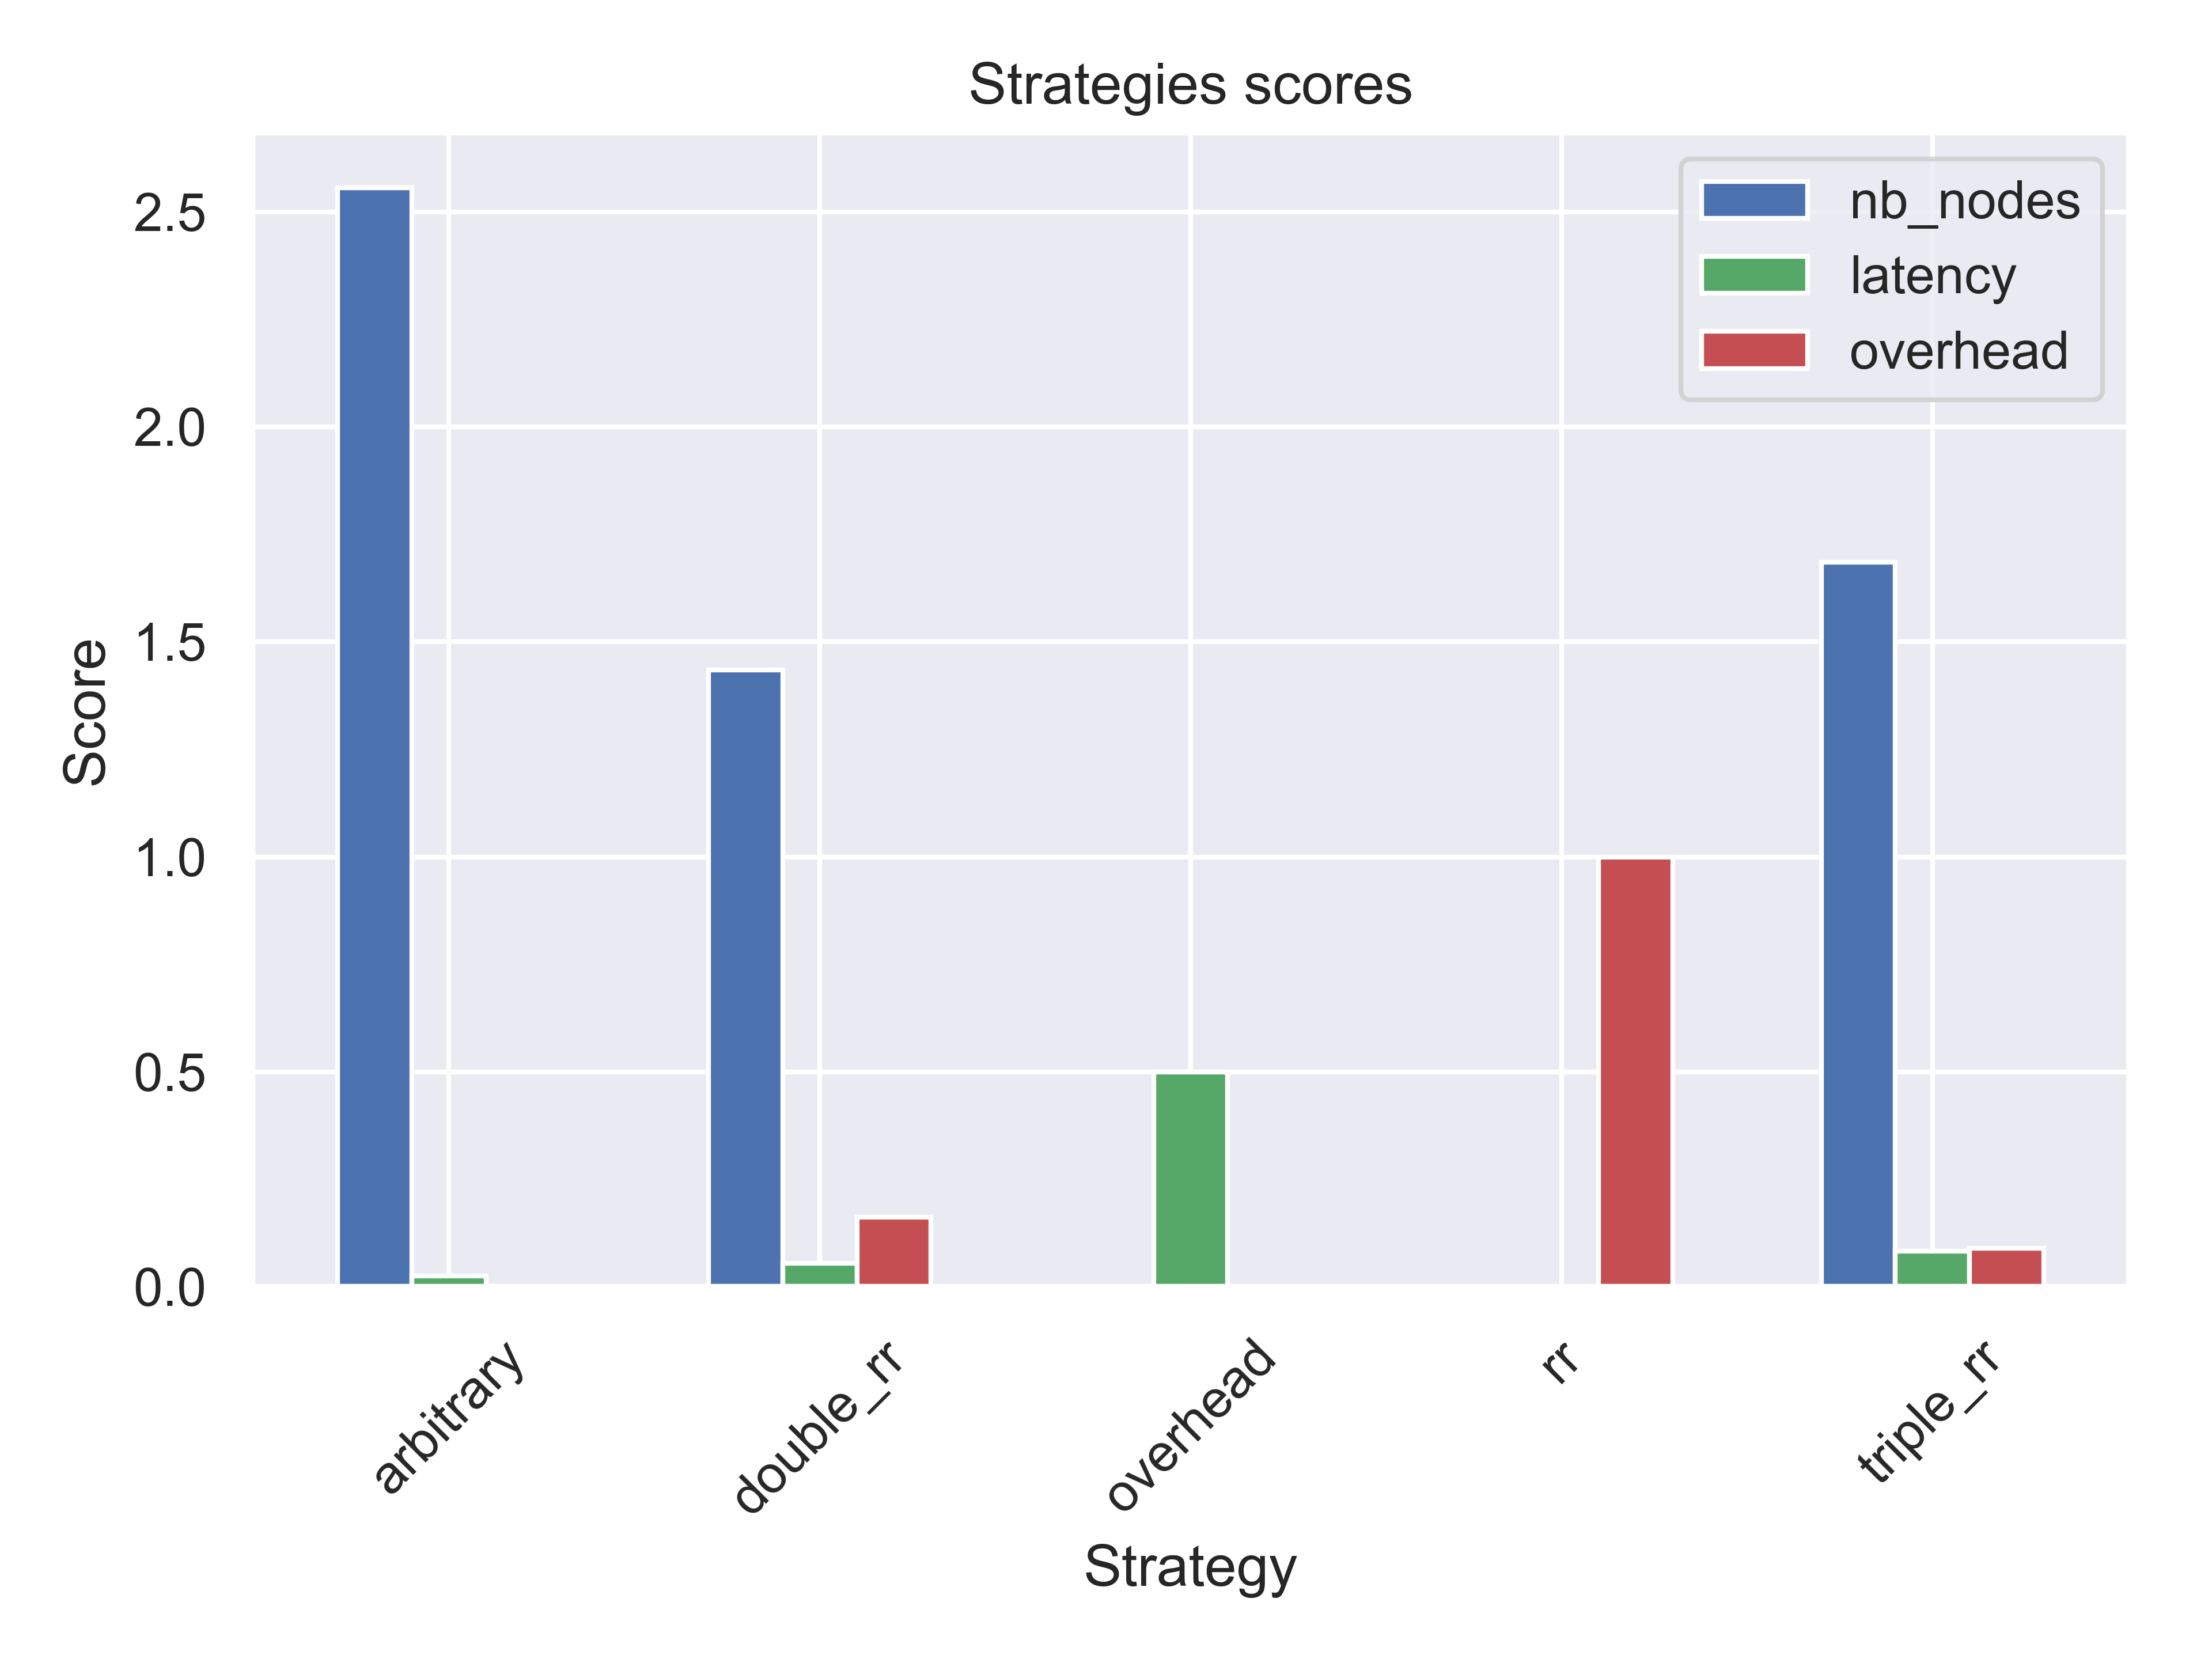
\includegraphics[width=0.8\columnwidth]{final_plot_basic_model}
    \captionsetup{justification=centering}
    \caption{Raw fitted calues for the simple model. The strategies are listed
    on the x-axis and their scores are plotted along the y-axis. \todo{prettify
    the x-axis and bar legend}}
    \label{fig:recapTestsPlot}
\end{figure}

%\begin{table}[H]
%    \centering{
%        \begin{tabular}{|c|c|c|c|}
%            \hline
%            Sending Strategy & \(s_n\) & \(s_l\) & \(s_o\) \\
%            \hline
%            Round-robin & 0.0 & 0.0 &
%            1.0\\
%            \hline
%            Double round-robin & 0.119 & 0.036 & 0.601\\
%            \hline
%            Triple round-robin & 0.404 & 0.082 & 0.401\\
%            \hline
%            Maximal overhead & 0.0 & 0.987 & 0.0\\
%            \hline
%            Arbitrary & 0.861 & 0.035 & 0.106\\
%            \hline
%        \end{tabular}
%        \captionsetup{justification=centering}
%        \caption{Raw fitted values for the simple model, rounded to the 3rd decimal}
%        \label{fig:recapTests}
%    }
%\end{table}
%
\begin{figure}[H] 
    \centering
    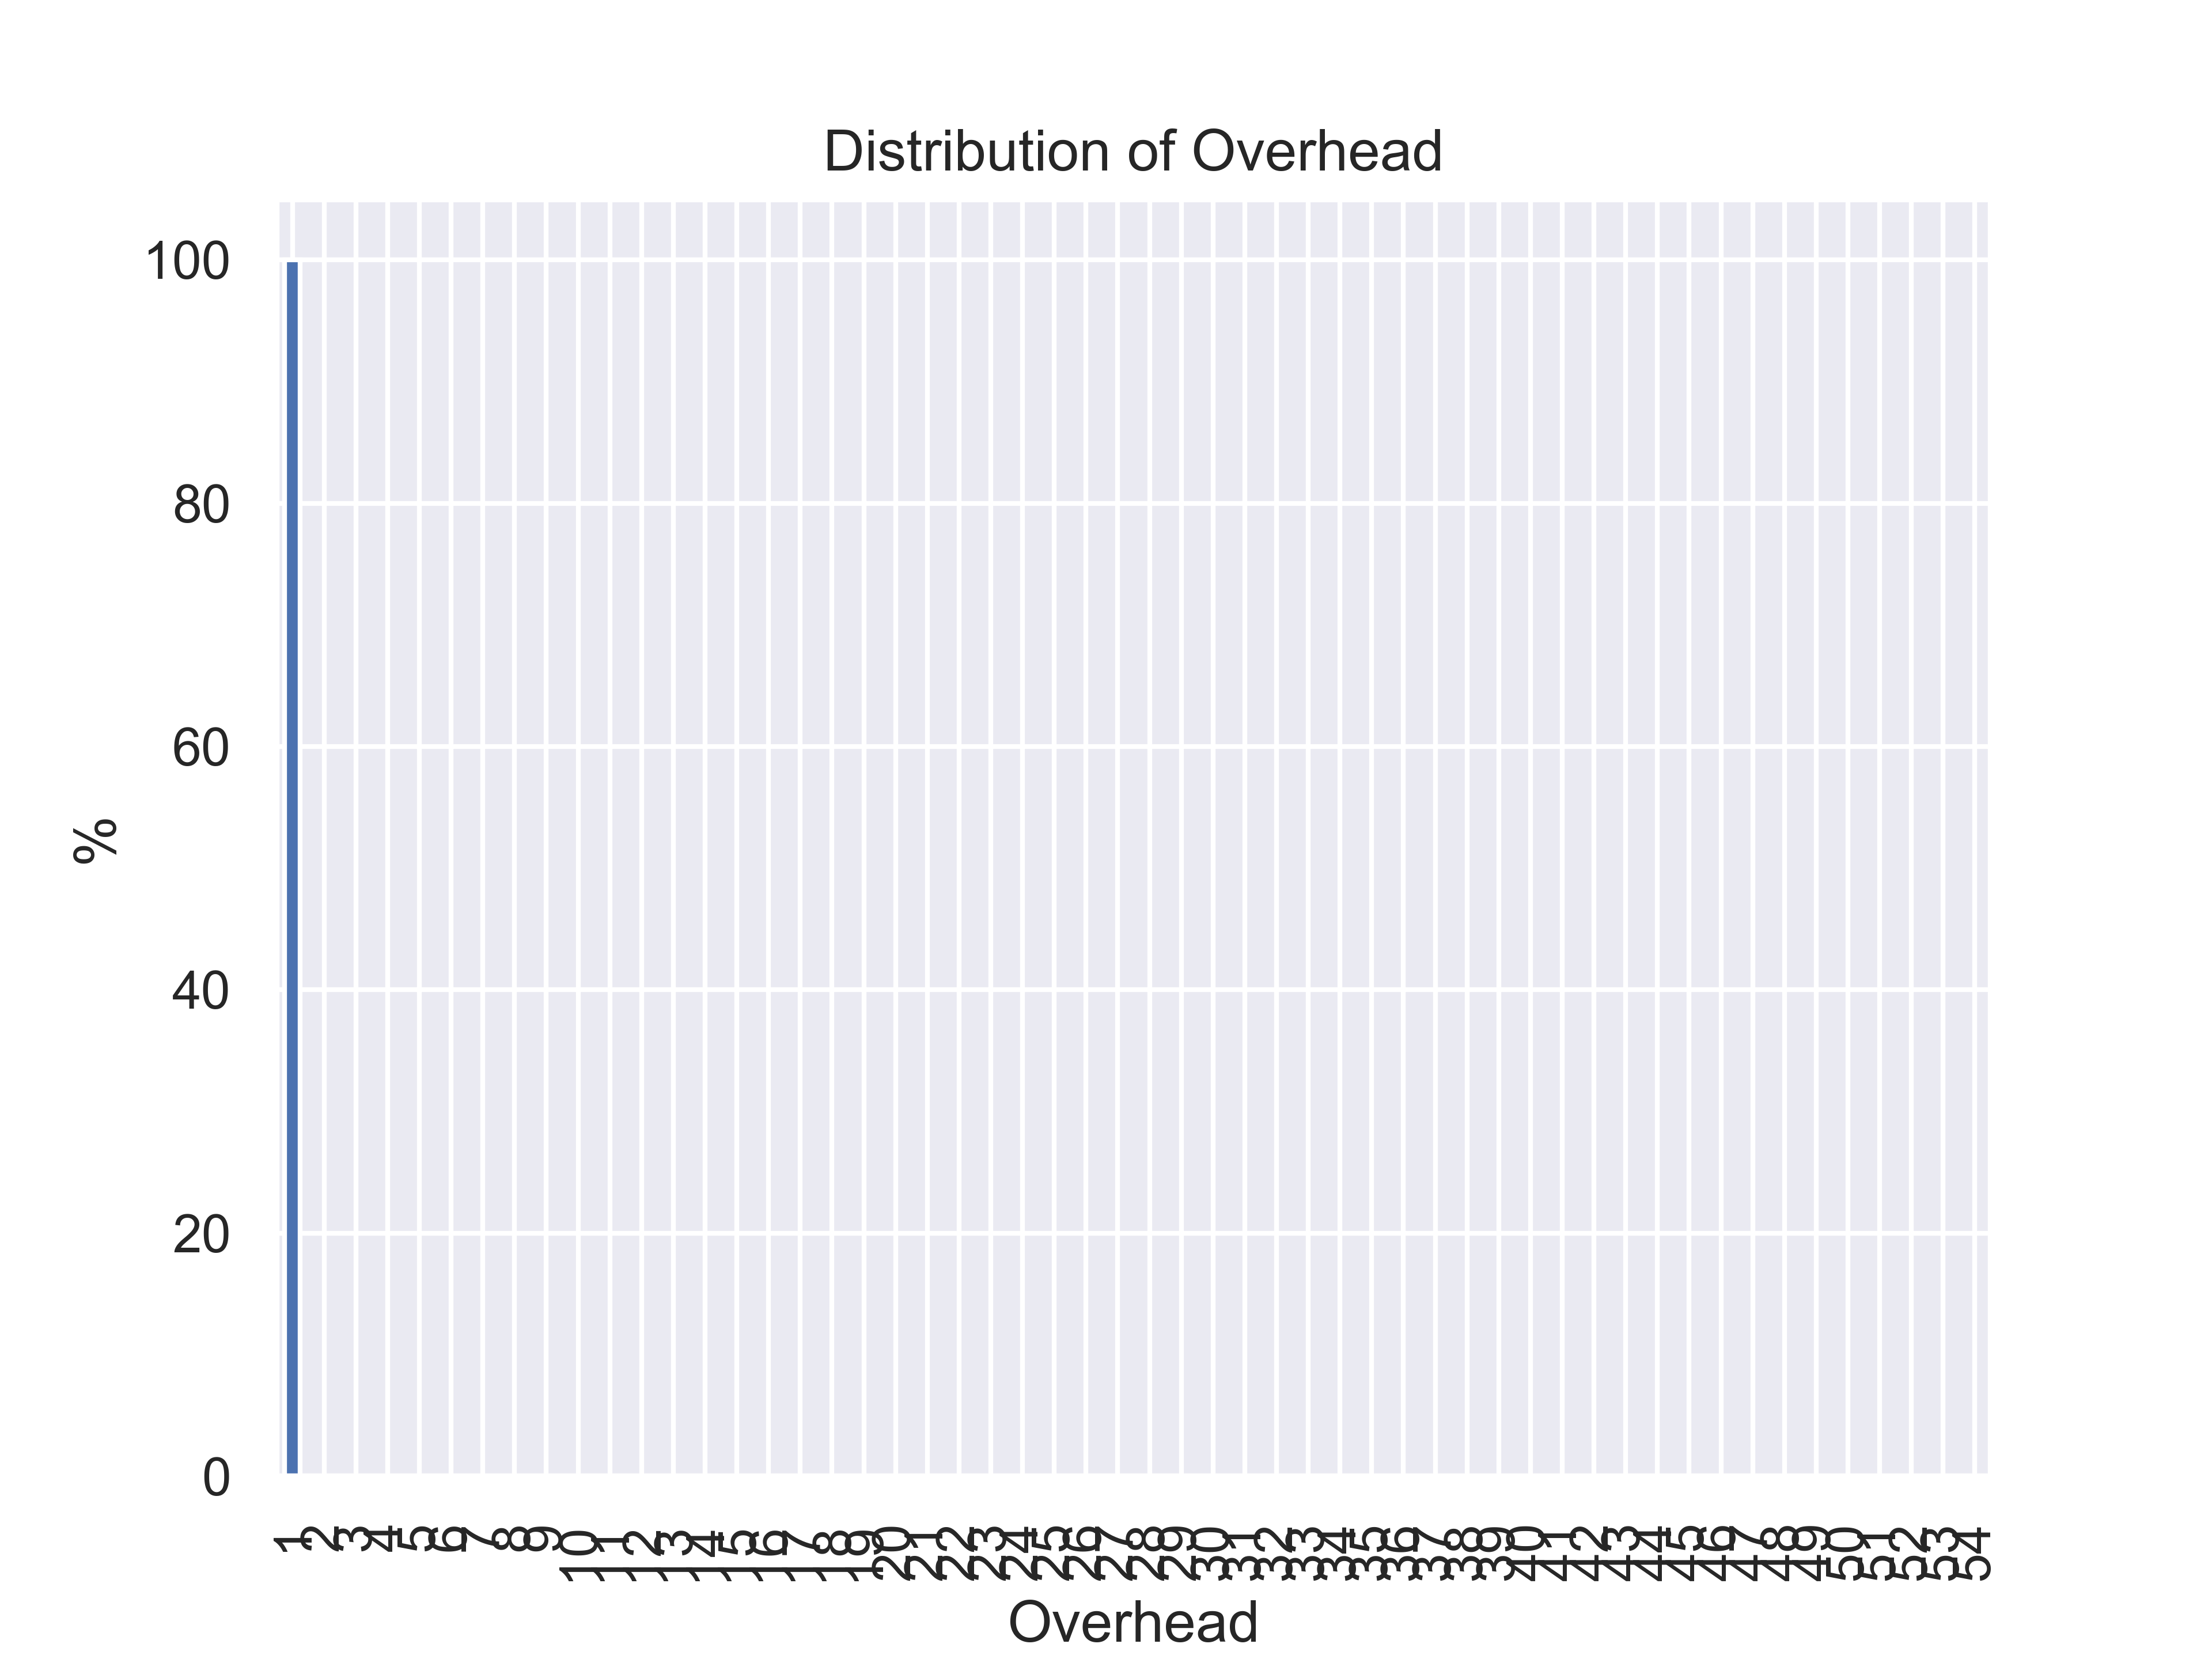
\includegraphics[width=0.8\columnwidth]{hist_overhead_rr_20_nodes_4_depth_all_receivers_gen_averages}
    \captionsetup{justification=centering}
    \caption{Histogram of the overhead. Round-robin and all receivers strategies}
    \label{fig:relOverheadLatencyRR}
\end{figure}



\subsection{Improvements of the basic model and new fitting}

\section{Analysis}
\todo{why the model is bad according to the number of nodes}

\todo{here will be a table containing all the fitted lines values and a
comparison and explanation of the behaviors that are observed}

\section{Future works}
